\documentclass[DIV16,twocolumn,10pt]{scrreprt}
\usepackage{paralist}
\usepackage{graphicx}
\usepackage[final]{hcar}

%include polycode.fmt

\begin{document}

\begin{hcarentry}{Kitchen Snitch server}
\report{Dino Morelli}
\status{stable, actively developed}
\participants{Betty Diegel}% optional
\makeheader

This project is the server-side software for Kitchen Snitch, a mobile application that provides health inspection scores, currently for the Raleigh-Durham area in NC, USA. The data can be accessed on maps along with inspection details, directions and more.

\vspace{5mm}

The back-end software provides a REST API for mobile clients and runs services to perform regular inspection data acquisition and maintenance.

\vspace{5mm}

Kitchen Snitch has been in development for over a year and is running on AWS. The mobile client and server were released for public use in April of 2016 after a beta-test period.

\vspace{5mm}

Some screenshots of the Android client software in action:

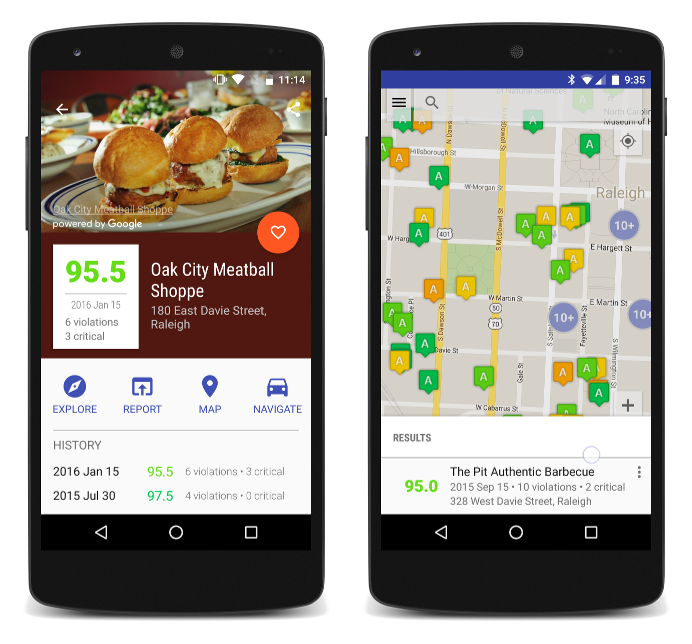
\includegraphics{ks_screenshots}

Getting Kitchen Snitch:

\vspace{5mm}

The mobile client can be installed from the Google Play Store \url{https://play.google.com/store/apps/details?id=com.honu.ksnitch}. There is also a landing page \url{http://getks.honuapps.com/}.

\vspace{5mm}

The Haskell server source code is available on darcshub at the URLs below.

\begin{kssrc}
 \item ks-rest \url{http://hub.darcs.net/dino/ks-rest}
 \item ks-download \url{http://hub.darcs.net/dino/ks-download}
 \item ks-library \url{http://hub.darcs.net/dino/ks-library}
\end{kssrc}

\end{hcarentry}

\end{document}
